\documentclass[11pt]{article}
\usepackage[utf8]{inputenc}

%%% PAGE DIMENSIONS
\usepackage{geometry}
\geometry{a4paper}

\usepackage{graphicx}

%%% PACKAGES
\usepackage{booktabs}
\usepackage{paralist}
\usepackage{verbatim}
\usepackage{subfig}
\usepackage{chngcntr}
\usepackage{tikz}
\usepackage[colorlinks = true,
            linkcolor = black,
            urlcolor  = blue,
            citecolor = blue,
            anchorcolor = blue]{hyperref}
\usepackage[spanish]{cleveref}
\usepackage{placeins}
\usepackage{float}

%%% HEADERS & FOOTERS
\usepackage{fancyhdr}
\pagestyle{fancy}
\renewcommand{\headrulewidth}{0pt}
\lhead{}\chead{}\rhead{}
\lfoot{}\cfoot{\thepage}\rfoot{}

%%% SECTION TITLE APPEARANCE
\usepackage{sectsty}
\allsectionsfont{\sffamily\mdseries\upshape}

%%% ToC (table of contents) APPEARANCE
\usepackage[nottoc,notlof,notlot]{tocbibind} % Put the bibliography in the ToC
\usepackage[titles,subfigure]{tocloft} % Alter the style of the Table of Contents
\renewcommand{\cftsecfont}{\rmfamily\mdseries\upshape}
\renewcommand{\cftsecpagefont}{\rmfamily\mdseries\upshape} % No bold!


\graphicspath{ {images/} }

\counterwithin*{figure}{section}
\counterwithin*{figure}{subsection}
\counterwithin*{figure}{subsubsection}

\counterwithin*{table}{section}
\counterwithin*{table}{subsection}
\counterwithin*{table}{subsubsection}

\addtolength{\cftfignumwidth}{2em}

\renewcommand{\thefigure}{
  \ifnum\value{subsection}=0
    \thesection.\arabic{figure}
  \else
    \ifnum\value{subsubsection}=0
      \thesubsection.\arabic{figure}
    \else
      \thesubsubsection.\arabic{figure}
    \fi
  \fi
}

\renewcommand{\thetable}{
  \ifnum\value{subsection}=0
    \thesection.\arabic{table}
  \else
    \ifnum\value{subsubsection}=0
      \thesubsection.\arabic{table}
    \else
      \thesubsubsection.\arabic{table}
    \fi
  \fi
}

%%% END Article customizations

%%% The "real" document content comes below...

\title{\Large Seguridad en Redes\\Practica 3.1}
\author{David Antuña Rodríguez\\Javier Carrión García}
\date{}

\begin{document}
  \raggedright

  \maketitle
  \newpage

  \par
  No tenemos la maquina Ubuntu porque no nos permitia descargarla.
  \section{Sniffing con Wireshark}
    \par
    Como no tenemos la maquina ubuntu solo hemos realizado los ping a metasploit. Aparecen dos
    paquetes ICMP, uno de echo request y otro de echo reply.

    \bigskip
    \par
    \textbf{Trama ICMP (request)}\\
    \hspace{5mm}IP origen 192.168.2.2\\
    \hspace{5mm}IP destino 192.168.1.1\\
    \hspace{5mm}MAC origen 08:00:27:66:bf:ba\\
    \hspace{5mm}MAC destino 08:00:27:43:e6:46\\

    \bigskip
    \par
    \textbf{Trama ICMP (reply)}\\
    \hspace{5mm}IP origen 192.168.1.1\\
    \hspace{5mm}IP destino 192.168.2.2\\
    \hspace{5mm}MAC origen 08:00:27:43:e6:46\\
    \hspace{5mm}MAC destino 08:00:27:66:bf:ba\\

    \bigskip
    \par
    La IP 192.168.2.2 y la MAC 08:00:27:66:bf:ba pertenecen a la maquina Host(atacante).\\
    La IP 192.168.1.1 y la MAC 08:00:27:43:e6:46 pertenecen a la maquina metasploitable.

  \section{Network scanning con nmap}
    \subsection{Descubrimieto de IPs}
      \par
      Utiliza una ARP request para cada una de las posibles direcciones de la red.\\
      Ambos escaneos detectan los mismos host pero el segundo tambien determina la MAC del router.

      \begin{figure}[H]
        \centering
        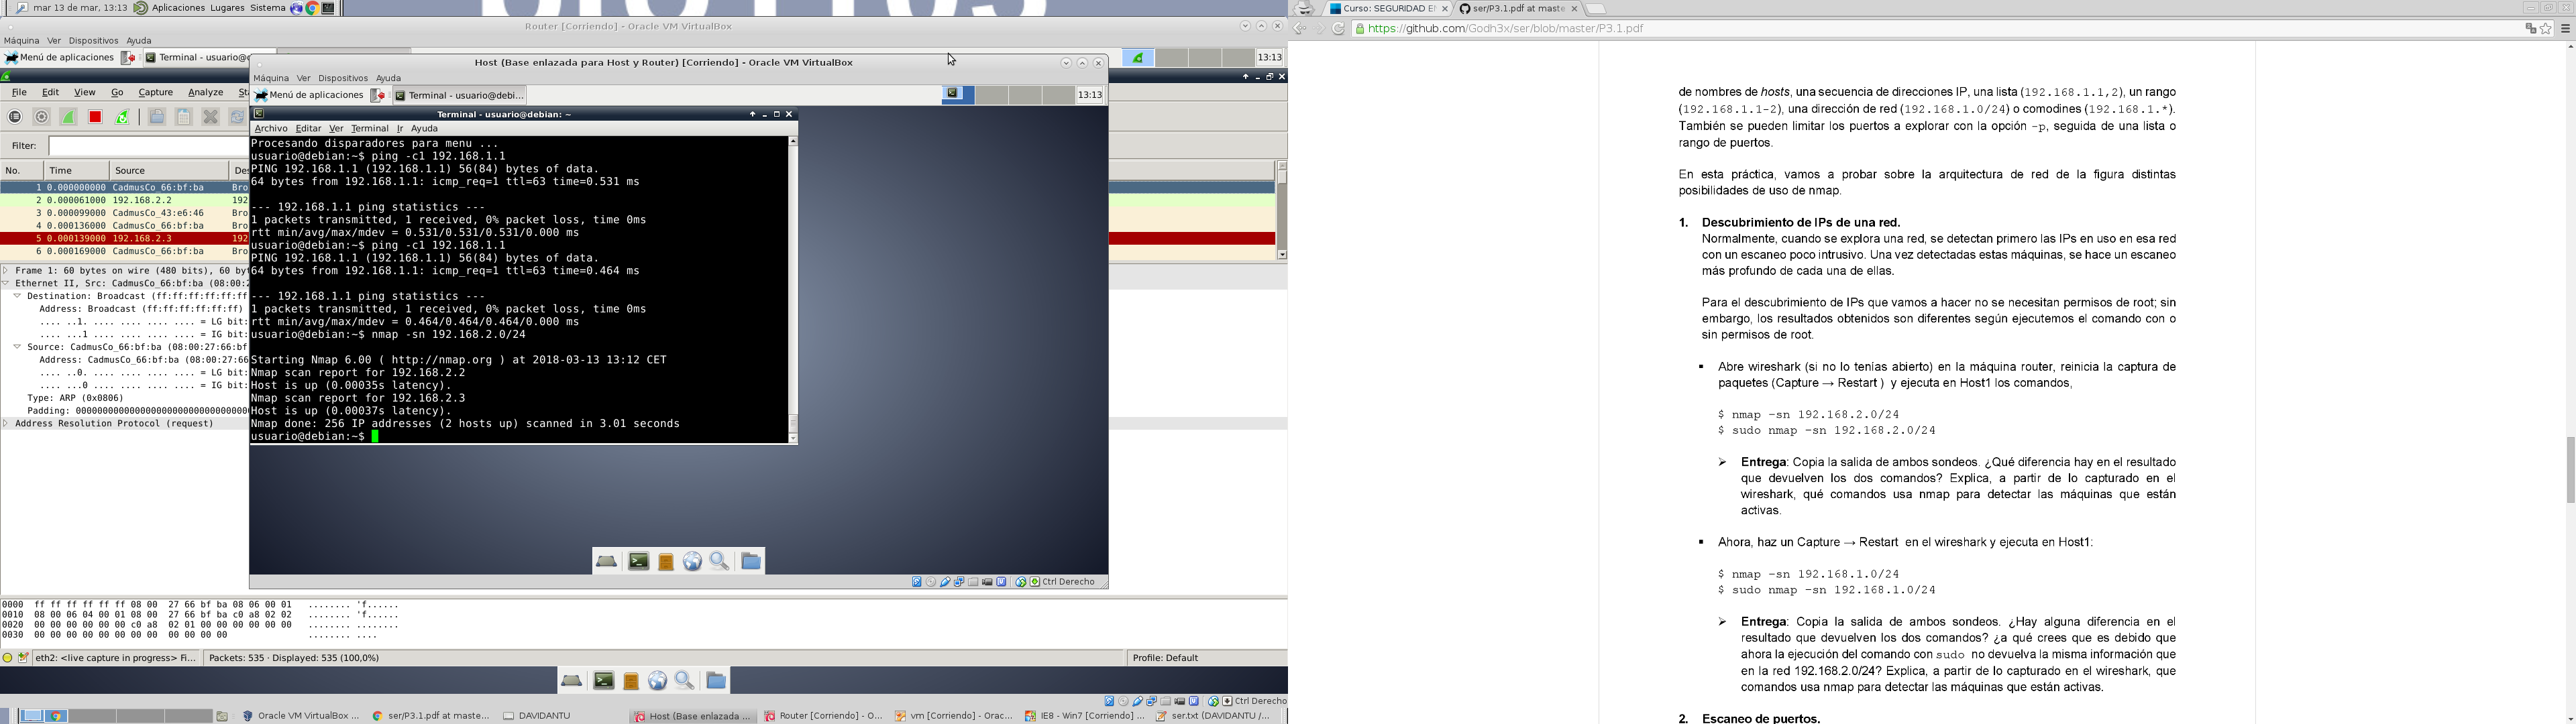
\includegraphics[width = \textwidth]{sondeo1}
        \caption{Sondeo red 2 sin sudo.}
      \end{figure}

      \begin{figure}[H]
        \centering
        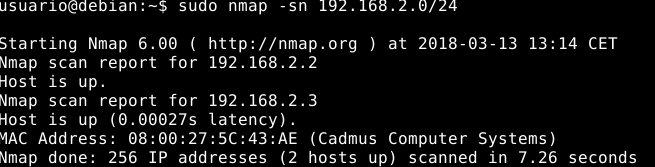
\includegraphics[width = \textwidth]{sondeo2}
        \caption{Sondeo red 2 con sudo.}
      \end{figure}

      \par
      No hay diferencia en sus resultados pero el segundo escaneo ha tardado más en completarse.\\
      Ahora no es capaz de devolver la MAC del router porque no forma parte de la red que está
      escaneando.

      \begin{figure}[H]
        \centering
        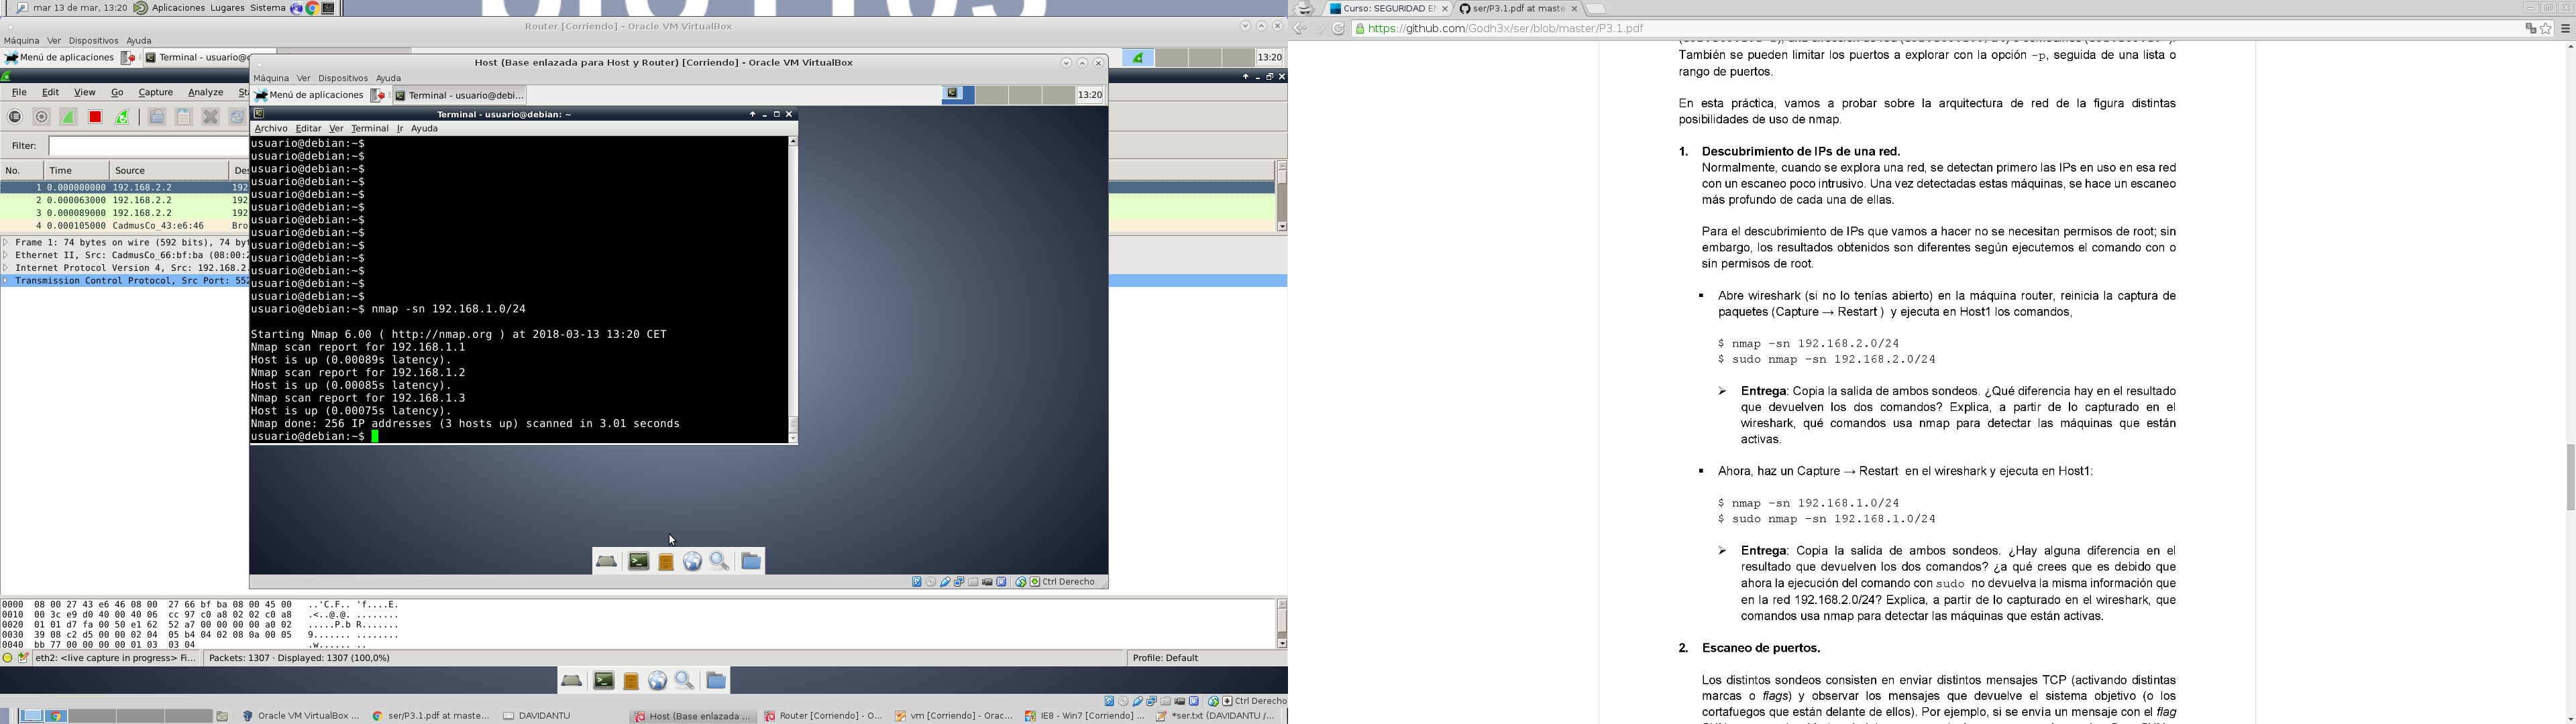
\includegraphics[width = \textwidth]{sondeo3}
        \caption{Sondeo red 1 sin sudo.}
      \end{figure}

      \begin{figure}[H]
        \centering
        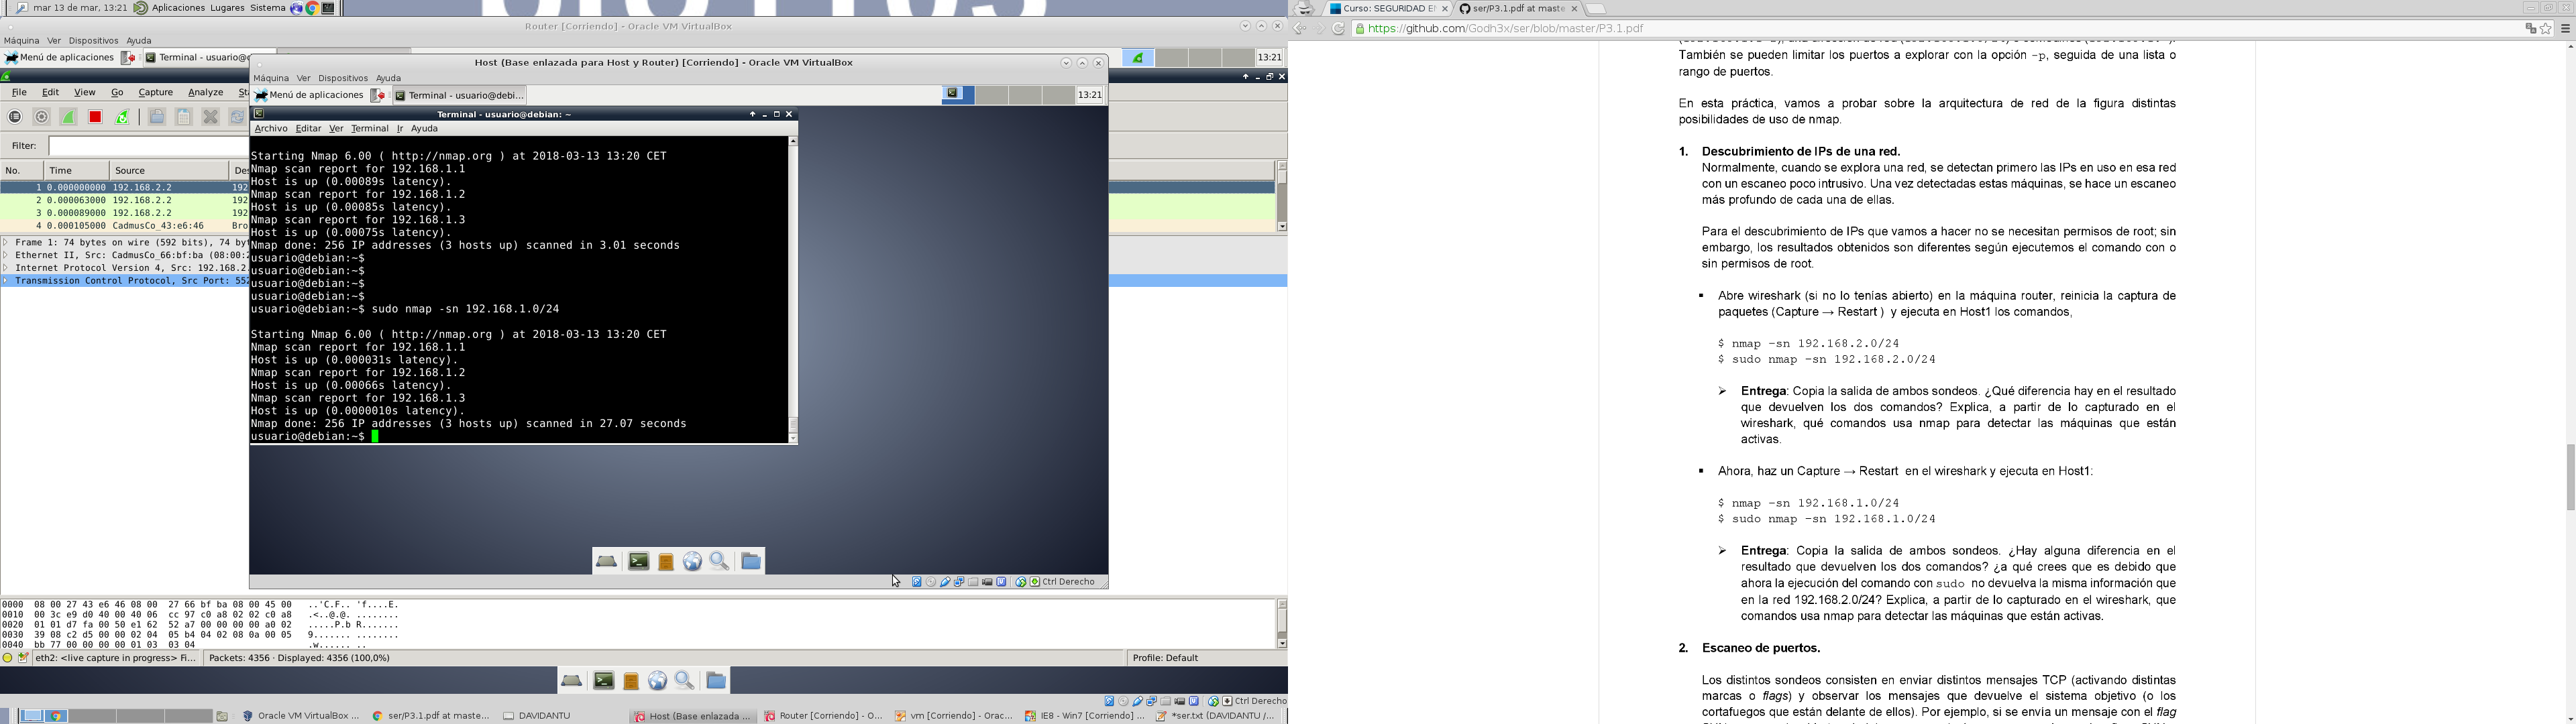
\includegraphics[width = \textwidth]{sondeo4}
        \caption{Sondeo red 1 con sudo.}
      \end{figure}
    \subsection{Escaneo de puertos}
      \par
      Cuando el puerto está abierto se contesta con un mensaje TCP que tiene las flags RST y ACK
      activas, no puede detectar puertos UDP porque el escaneo es por TCP.

      \begin{figure}[H]
        \centering
        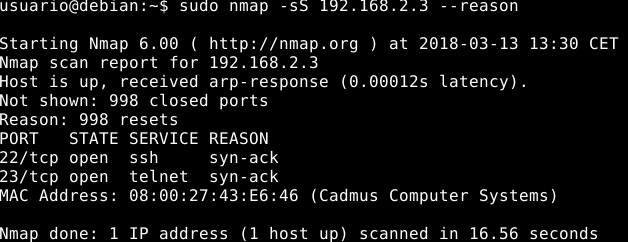
\includegraphics[width = \textwidth]{sondeo5}
        \caption{sudo nmap $-$sS 192.168.2.3 $-$$-$reason}
      \end{figure}

      \begin{figure}[H]
        \centering
        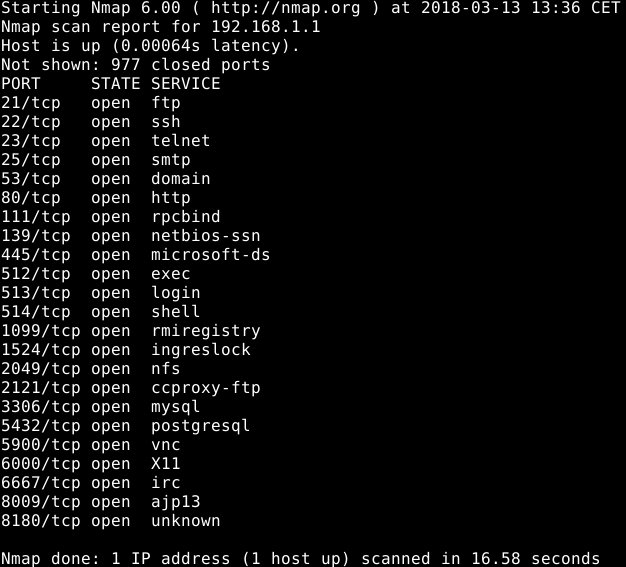
\includegraphics[width = .9\textwidth]{sondeo7}
        \caption{sudo nmap $-$sS 192.168.1.1}
      \end{figure}

      \begin{figure}[H]
        \centering
        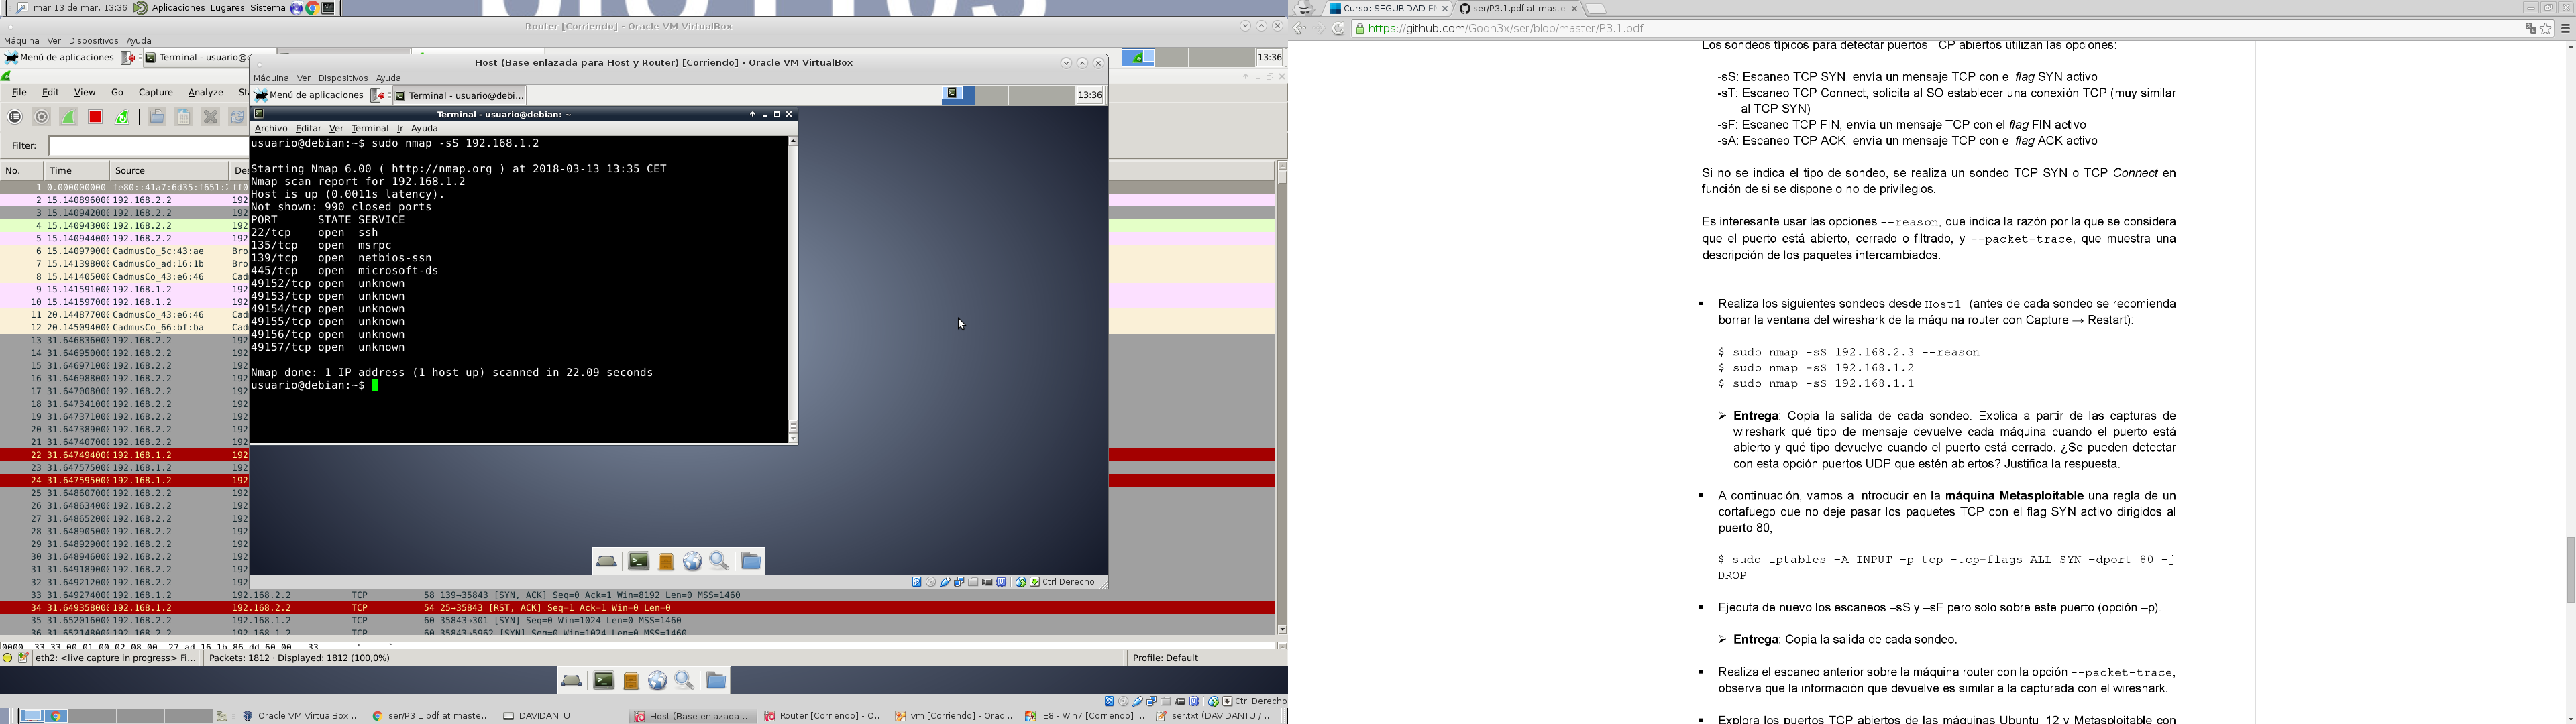
\includegraphics[width = .9\textwidth]{sondeo6}
        \caption{sudo nmap $-$sS 192.168.1.2}
      \end{figure}

      \par
      Repetimos los escaneos para el puerto 80 despues de añadir la nueva regla.

      \begin{figure}[H]
        \centering
        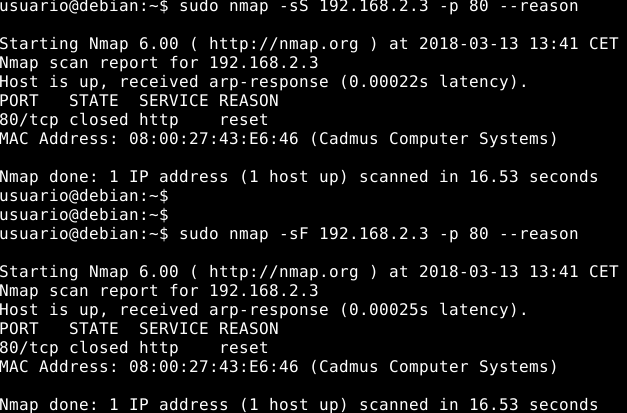
\includegraphics[width = .9\textwidth]{sondeo8}
        \caption{sudo nmap $-$sS 192.168.2.3 $-$p 80 $-$$-$reason.}
      \end{figure}

      \begin{figure}[H]
        \centering
        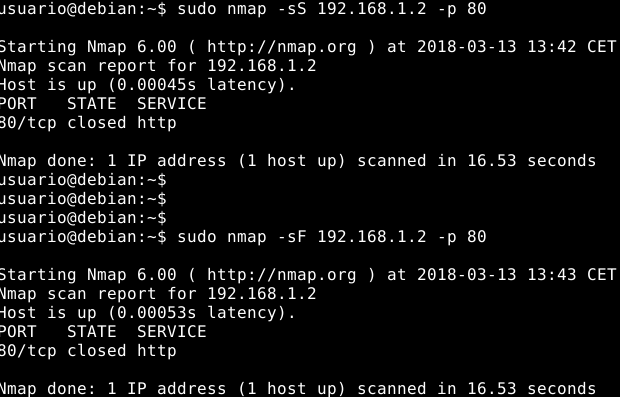
\includegraphics[width = .9\textwidth]{sondeo9}
        \caption{sudo nmap $-$sS 192.168.1.2 $-$p 80}
      \end{figure}

      \begin{figure}[H]
        \centering
        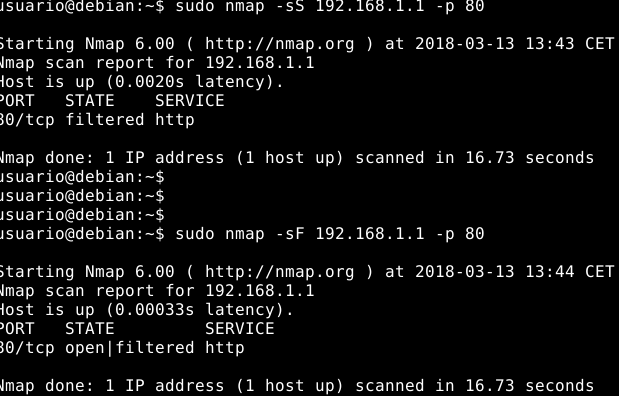
\includegraphics[width = .9\textwidth]{sondeo10}
        \caption{sudo nmap $-$sS 192.168.1.1 $-$p 80}
      \end{figure}

      \newpage
      \par
      Exploracion de los puertos TCP en metasploitable.

      \begin{figure}[H]
        \centering
        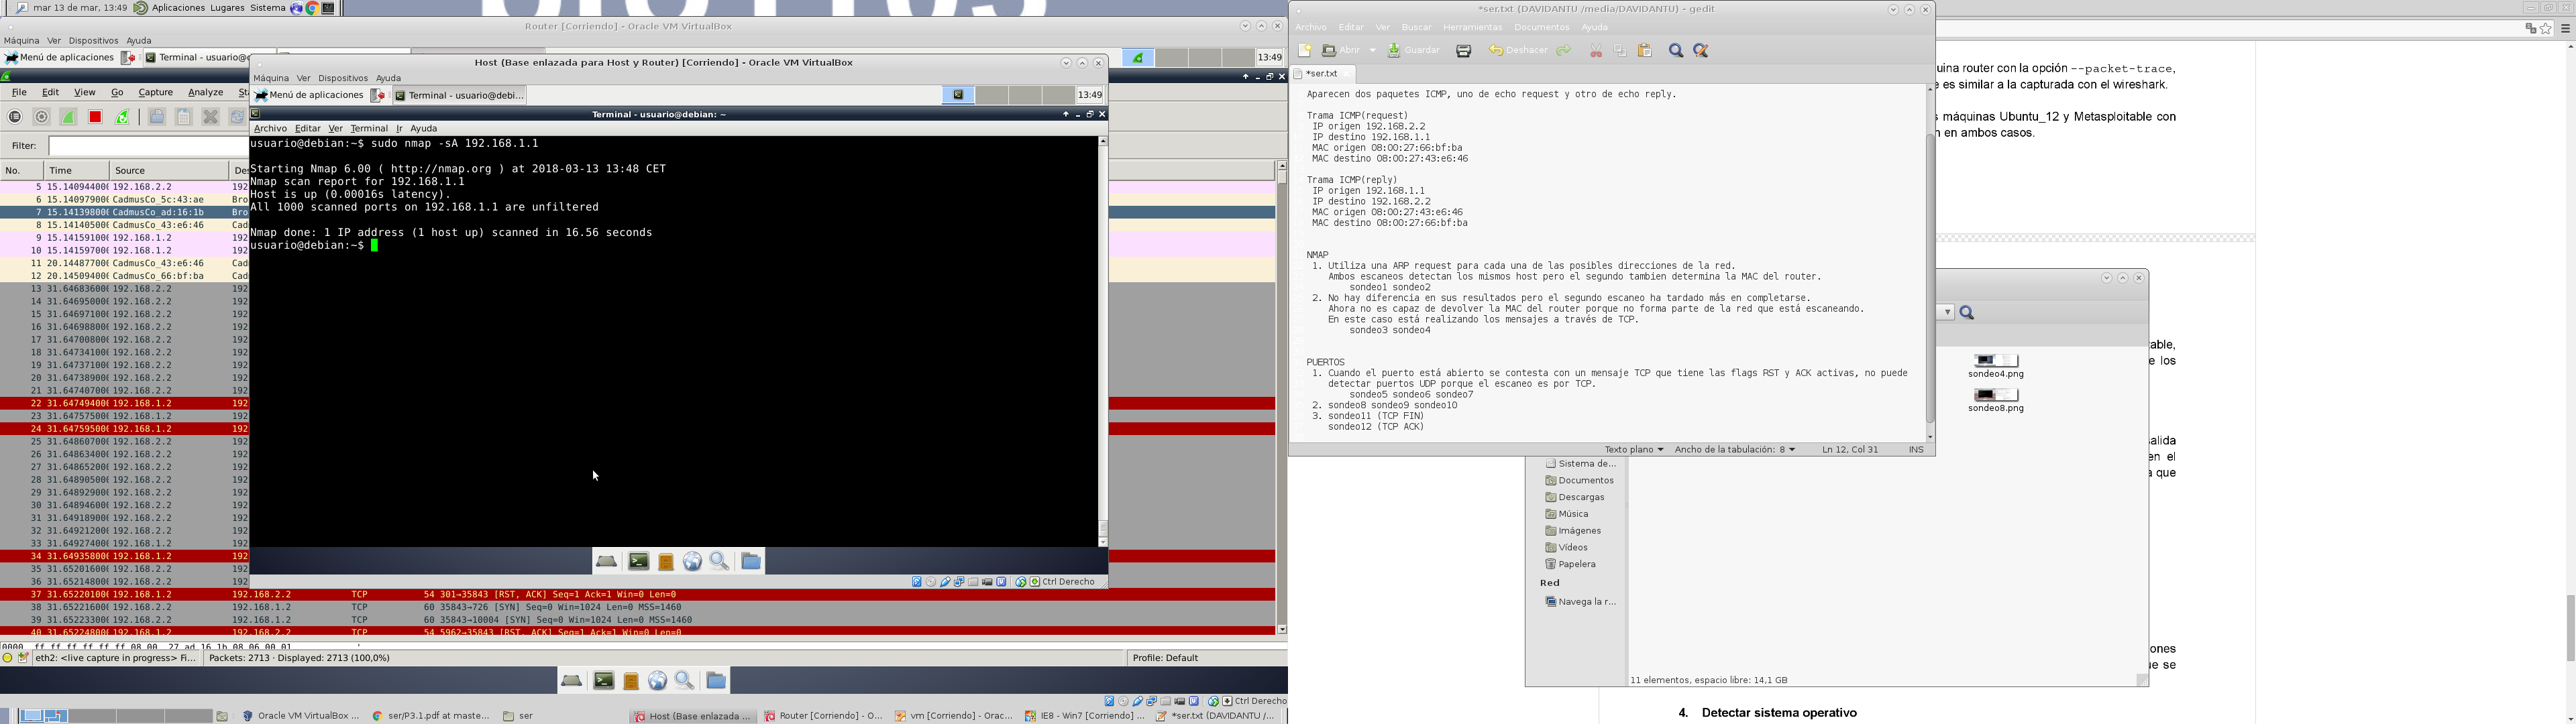
\includegraphics[width = \textwidth]{sondeo12}
        \caption{Sondeo TCP ACK.}
      \end{figure}

      \begin{figure}[H]
        \centering
        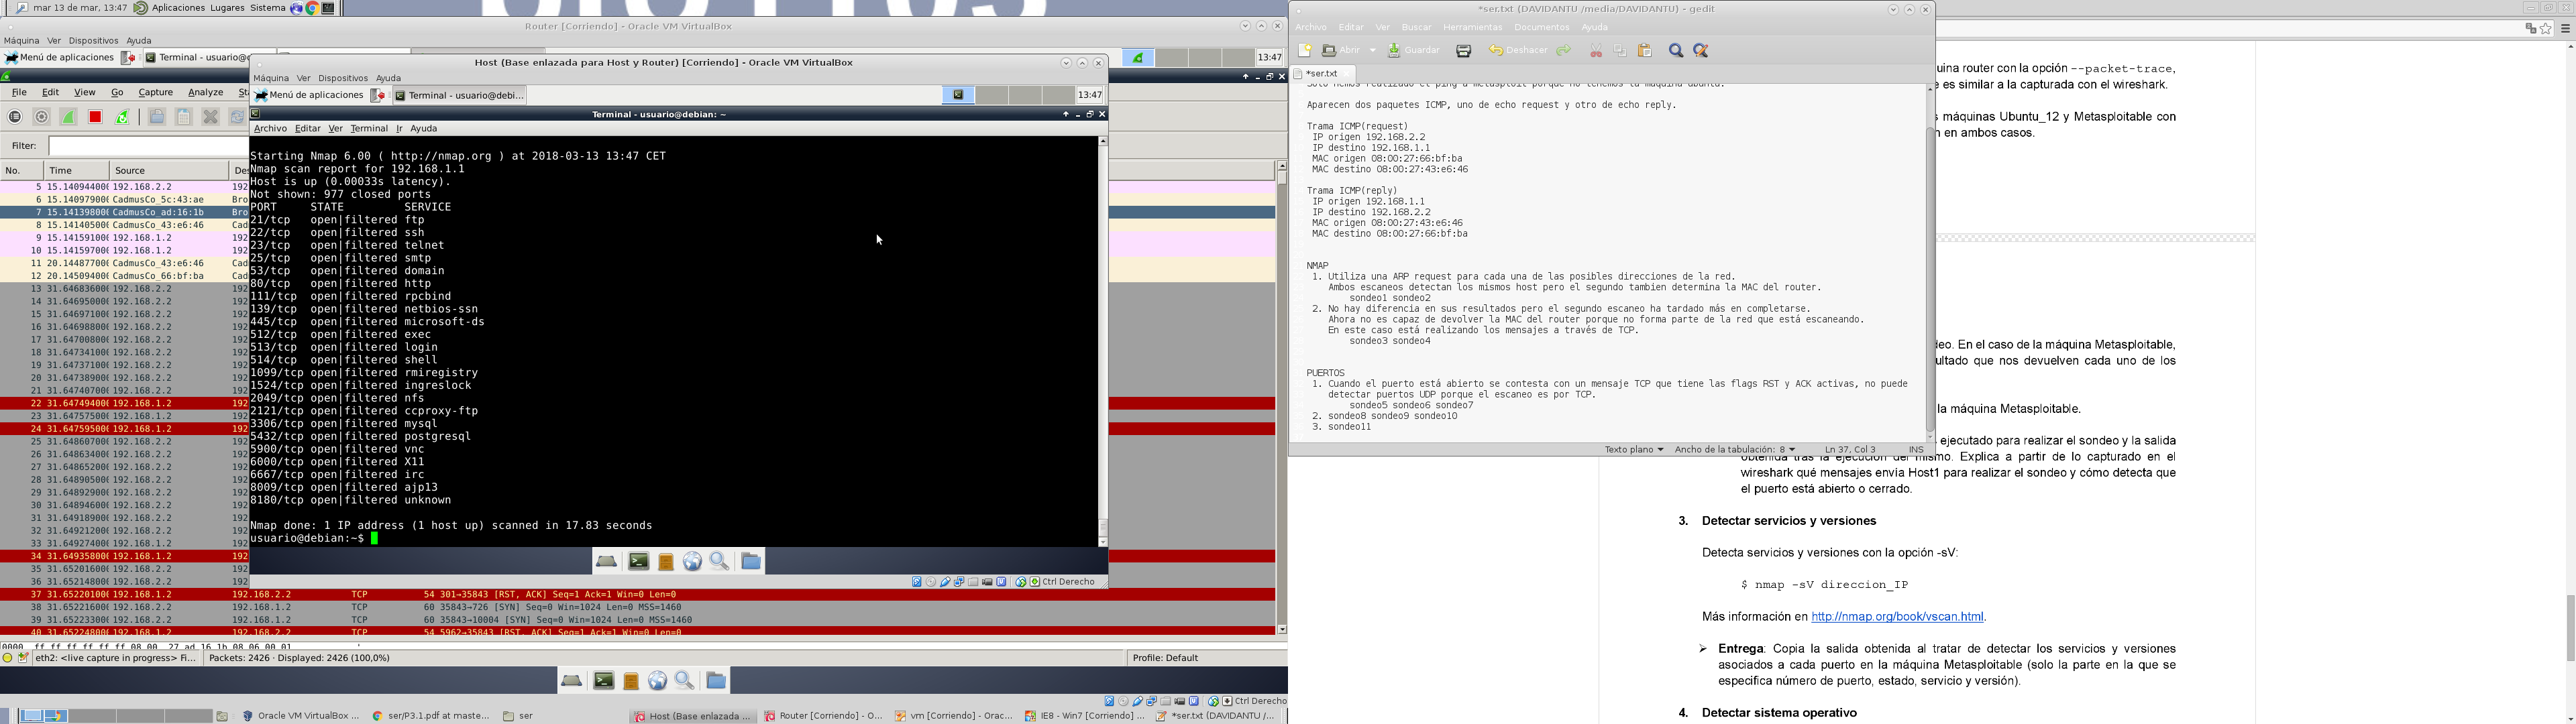
\includegraphics[width = \textwidth]{sondeo11}
        \caption{Sondeo TCP FIN.}
      \end{figure}

    \subsection{Detectar servicios y versiones}
      \begin{figure}[H]
        \centering
        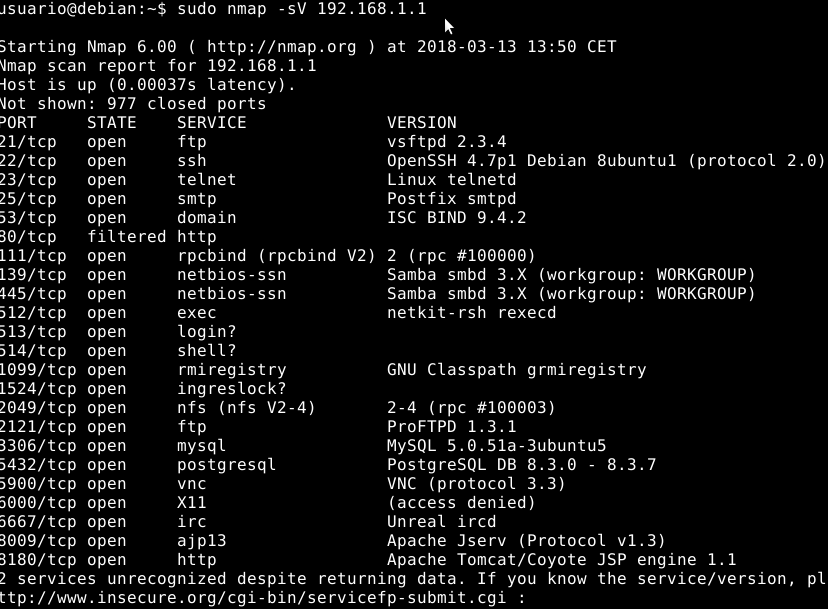
\includegraphics[width = \textwidth, height = 10cm]{sondeo13}
        \caption{Deteccion de servicios en metasploit.}
      \end{figure}

      \begin{figure}[H]
        \centering
        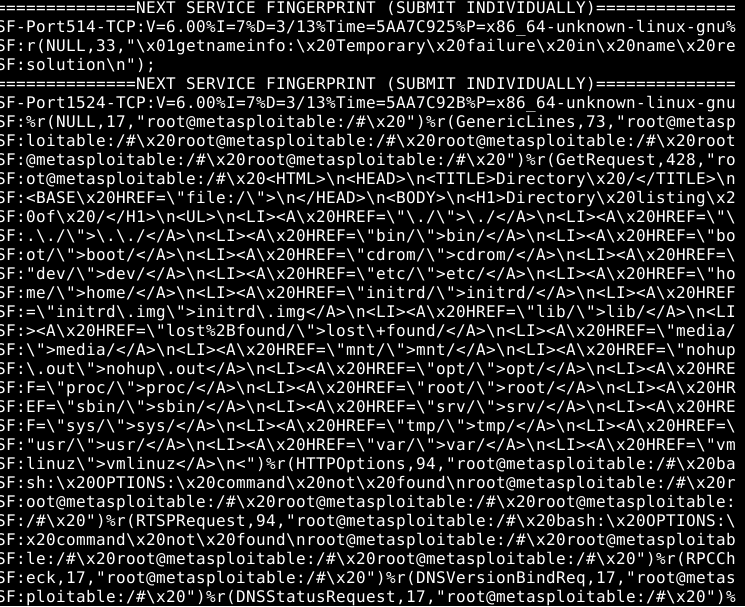
\includegraphics[width = \textwidth, height = 7cm]{sondeo14}
        \caption{Deteccion de servicios en metasploit (2).}
      \end{figure}

    \subsection{Detectar sistema operativo}
      \par
      La maquina de Windows se cayó y no pudimos ejecutar este apartado en ella.

      \begin{figure}[H]
        \centering
        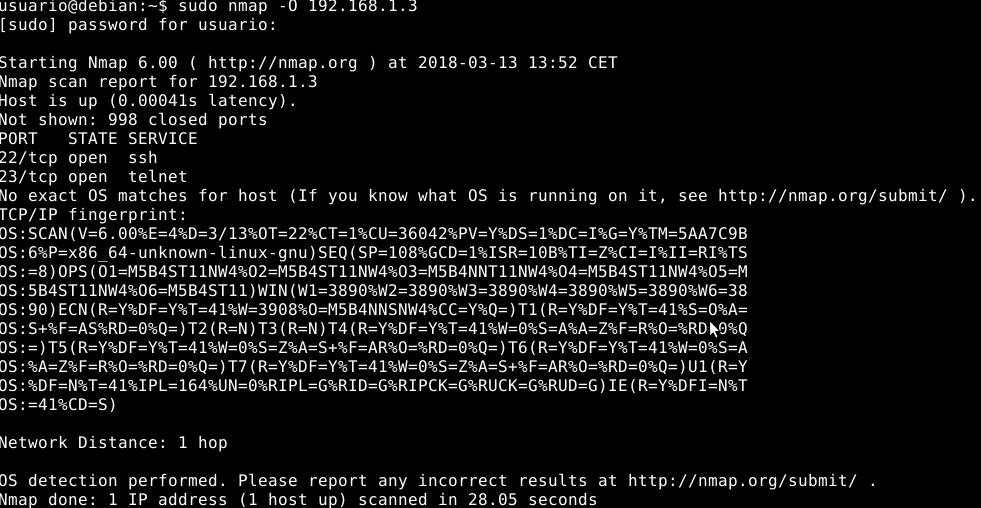
\includegraphics[width = \textwidth]{sondeo15}
        \caption{Sondeo SO router.}
      \end{figure}

      \begin{figure}[H]
        \centering
        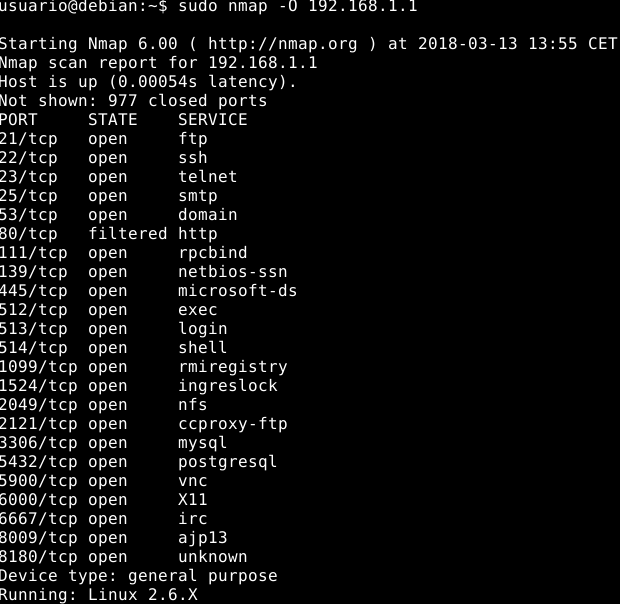
\includegraphics[width = \textwidth]{sondeo16}
        \caption{Sondeo SO metasploitable.}
      \end{figure}
\end{document}
